\documentclass{article} 
\usepackage{amsmath}  
\usepackage{amsthm, amssymb}
\usepackage[a4paper,left=25mm,right=25mm,top=30mm,bottom=30mm]{geometry}
\usepackage{fancyhdr}
\usepackage{titlesec}
\usepackage{enumerate}
\usepackage{graphicx} 
\usepackage[dvipsnames]{xcolor}
\usepackage{transparent} 
\usepackage{parskip}
\usepackage{tikz} 
\usepackage[condensed,light,math]{iwona}
\usepackage[T1]{fontenc}

\title{combinatorics exercises} 
\author{emilianna monami louise limlengco} 
\date{\today} 

\fboxsep=4pt
\renewcommand{\footnoterule}{\vfill\kern-3pt \hrule width 0.4\columnwidth\kern2.6pt} %yoinked from LSE
\renewcommand{\labelitemi}{$\rightarrow$}
\renewcommand{\labelenumi}{\colorbox{pink}{\textbf{\arabic{enumi}}}}
\renewcommand{\labelenumii}{\transparent{0.5}\colorbox{CornflowerBlue}{\transparent{1.0}\textbf{\alph{enumii}}}}

\newcommand{\multibinom}[2]{
  \left(\!\!\middle(\genfrac{}{}{0pt}{}{#1}{#2}\middle)\!\!\right)} %yoinked from LSE

\newenvironment{solution}
  {\renewcommand\qedsymbol{$\blacksquare$}\begin{proof}[Solution]}
  {\end{proof}}

\begin{document}

\section*{How to Use this Reviewer}
Hello! This is a compilation of solved exercises for module 3 of MATH 51.3. All of these exercises are taken straight from sir Aldrich's course notes, so you can expect tests 
to be very similar to the items given. However, there are certain items that are much more difficult than what he expects us to do, and are mostly for nerds like me to geek out about 
on documents like these. I'll note when these items show up, so that you don't spend energy that you don't really need or want to trying to understand them.\par Normal items will look like this:\begin{enumerate} 
    \item A very easy math problem. What's 1 + 1?
\end{enumerate} 
whereas difficult problems will be soulless, like this:\begin{enumerate}\setcounter{enumi}{1}
    \renewcommand{\labelenumi}{\fcolorbox{magenta}{white}{\textbf{\arabic{enumi}}}}
    \item A very difficult math problem. Prove that $\displaystyle \binom{2n}{n} < 2^{2n-2},~\forall n \geq 5$ using induction. 
\end{enumerate} I might also include warnings in my \textbf{Nerd Interjections!}\par
\parindent=25pt \begin{minipage}[t]{.14\textwidth}
    \vspace{0pt}
    \includegraphics[width=2cm]{nerd_maddy.png} 
\end{minipage}%
\fbox{
\begin{minipage}[t]{.76\textwidth}
    \vspace{0pt}
    \textbf{Nerd Interjection!}\footnote{Image from @Ellem\_\_ on Twitter.} These sections are for me to remind you of some necessary information to solve the problems, elaborate on 
    something that I think isn't all that clear with just pure math symbols, give a helpful theorem, be an annoying piece of shit, anything, really! Just think of it as a tips and tricks section. 
\end{minipage}%
}\parindent=0pt \par I also have another section called \textbf{Can we Prove it?} (unfortunately lacking a cute picture to go along with it), where I include some interesting, not really necessary, but 
nonetheless relevant proofs. So far, these two are my only two gimmicks, but I might add more in the future.\par
\fbox{\begin{minipage}[t]{0.98\textwidth}
    \vspace{0pt} 
    \textbf{Can we Prove it?} This is just a random proof I yoinked from our homeworks.\begin{proof} 
        ($ \implies $) Let $ x \in (A \cap B) \setminus C $. Then, $ x \in (A \cap B)$ and $ x \notin C $. \\
        \phantom{($ \implies $)} Since $x \in (A \cap B)$, $ x \in A$ and $ x \in B$. \\
        \phantom{($ \implies $)} Since $x \in A$ and $x \notin C$, $x \in (A \setminus C) $. \\
        \phantom{($ \implies $)} Since $x \in B$ and $x \notin C$, $x \in (B \setminus C) $. \\
        \phantom{($ \implies $)} Thus, $x \in (A \setminus C) \cap (B \setminus C) $. \\ 
        \\
        ($ \impliedby $) Let $ x \in (A \setminus C) \cap (B \setminus C) $. Then, $ x \in (A \setminus C) $ and $ x \in (B \setminus C) $. \\ 
        \phantom{($ \impliedby $)} Since $ x \in (A \setminus C) $, $ x \in A $ and $ x \notin C $. \\
        \phantom{($ \impliedby $)} Since $ x \in (B \setminus C) $, $ x \in B $ and $ x \notin C $. \\
        \phantom{($ \impliedby $)} Since $ x \in A $ and $ x \in B $, $ x \in (A \cap B) $. \\
        \phantom{($ \impliedby $)} Thus, $ x \in (A \cap B) \setminus C $. \\
        \\ 
        Since both sides of the conditional are true, it holds that $ (A \cap B) \setminus C = (A \setminus C) \cap (B \setminus C) $. 
    \end{proof} 
\end{minipage}%
}\par
Finally, there are blue boxes to indicate when instructions aren't obvious from the question itself, or if there are similar items that can be grouped together.\par
\parindent=25pt \transparent{0.5}
    \colorbox{CornflowerBlue}{
    \transparent{1.0}
    \begin{minipage}[c]{0.9\textwidth}
        \centering
        For items \#7 to \#12, we need to reevaluate our life decisions.
    \end{minipage}
    }\transparent{1.0}\parindent=0pt \par 
It's very important to note that this is a \textit{work in progress!} I am human, and I will make mistakes, and I cannot finish doing all the exercises within the span of one day. If you spot anything wrong, 
please feel free to message me; I will correct it as soon as possible.\par
As a final note, these are not replacements for the modules/paying attention in class, these are supplements for them. I won't explain all the topics here, and I'll assume that you at least have 
read the basics, so don't treat these reviewers as your only source of information. Sir Aldrich spends a lot of time on his handouts, they're really good! (except when they're wrong) With that, though, I think 
I've covered all pertinent points. Good luck, and happy studying!
\pagebreak 

\section*{3.1.1: Counting Problems} 
\textit{For these problems in particular, your solutions needn't be anywhere near this long; I've just explained the process in case it's unclear to anyone reading. Also because I love talking to myself on documents.}
\begin{enumerate}
    \item How many length-9 binary strings are there?\begin{solution} 
        Since there are only two options per digit of a binary string (1 or 0), we can simply do $ 2 \cdot 2 \cdot \hdots \cdot 2$ a total of nine times, or $2^9$, giving us $512$ different strings of length $9$. 
    \end{solution} 
    \item How many length-9 binary strings with exactly four 1's are there?\begin{solution} 
        Again, since there are only two options per digit of a binary string (1 or 0), and we want exactly four 1's, we can simply do $\binom{9}{4}$. Alternatively, you could count the number of ways you could make a string with 
        five 0's instead, which is $\binom{9}{5}$. [Recall that $\binom{n}{k} = \binom{n}{n-k}$]. This gives us 126 possible strings of length 9 with exactly four 1's. 
    \end{solution}%
    \begin{minipage}[t]{.14\textwidth}
        \vspace{0pt}
        \includegraphics[width=2cm]{nerd_maddy.png} 
    \end{minipage}%
    \fbox{
    \begin{minipage}[t]{.76\textwidth}
        \vspace{0pt}
        \textbf{Nerd Interjection!}\footnote{Image from @Ellem\_\_ on Twitter.} Notice how we used the product rule for \#1 but $\binom{n}{k}$ for \#2. Why'd we use two separate techniques for problems that look basically the same? 
        Well, in general, any solution that involves only two options can be solved with $\binom{n}{k}$. Even the first one! Solving \#1 like that would just involve adding the ways to count all possible amounts of 1's (or 0's) 
        that there are, so $\binom{9}{0} + \binom{9}{1} + \hdots + \binom{9}{9}$. Thus, \[
            \sum_{k=0}^{n} \binom{n}{k} = 2^n.     
        \]
    \end{minipage}%
    }\begin{solution} 
        An alternative solution for \#2 would be to start with the total amount of strings (since we already know its 512 from \#1) and subtract the ones that don't satisfy our conditions, 
        which would be the ones with $\neq$ four 1's. To get this number, we add $\binom{9}{0} + \binom{9}{1} + \hdots + \binom{9}{3} + \binom{9}{5} + \hdots + \binom{9}{9}$, giving us $512 - 386 = 126$. However, this solution 
        is much longer and I don't like it. 
    \end{solution} 
    \item  How many length-7 ternary strings begin with either 1 or 01? \begin{solution} 
        In this problem, we can see two cases. The first case is all ternary strings that start with 1, and the second case is all ternary strings that start with 01. Since the starting digit 
        is different in both cases, we can be sure that these two are distinct and exclusive from each other. Thus, finding the total would just be equivalent to solving each case individually 
        and adding them together. 
        \begin{itemize}
            \item Case 1: The strings that start with 1 can be counted by fixing the first digit, then multiplying the possibilities for the rest. Thus, $1 \cdot 3^6 = 729$ strings. 
            \item Case 2: The strings that start with 01 can be counted by fixing the first two digits, then multiplying the possibilities for the rest. Thus, $1 \cdot 1 \cdot 3^5 = 243$ strings. 
        \end{itemize} Adding these together gives us 972 strings of length 7 that start with either 1 or 01. 
    \end{solution} 
    \item How many length-7 ternary strings begin with 1 or end with 1?\begin{solution} 
        In this problem, we can also see two cases, the first case being all those that start with 1 and the second case being all thsoe that end with 1. However, these cases are not exclusive 
        from each other, as there are ternary strings that both start and end with 1. Thus, if we were to treat them individually, then there would be some double-counting occurring. Our cases can 
        then be edited into those that start with 1, and those that end with 1 but do not start with 1 (or vice-versa; the process will be the same). 
        \begin{itemize} 
            \item Case 1: The strings that start with 1 can be counted by fixing the first digit, then multiplying the possibilities for the rest. Thus, $1 \cdot 3^6 = 729$ strings.
            \item Case 2: The strings that end with 1 and do not start with 1 can be counted by fixing the last digit, then allowing only two options for the first digit, then multiplying the possibilities for the rest. 
            Thus, $2 \cdot 3^5 \cdot 1 = 486$ strings. 
        \end{itemize} Adding these together gives us 1215 strings of length 7 that either start with 1 or end with 1. 
    \end{solution} 
    \item How many length-5 ternary strings contain 1?\begin{solution} 
        In this problem, we can identify five distinct cases. We can fix the first digit as 1, then count the number of strings that fulfill that condition. Then, we move and 
        fix the second digit as 1, but we exclude all the strings that have the first digit as 1 since we already counted them in the first case. We then continue this for all five digits. 
        \begin{itemize} 
            \item Case 1: The strings that have 1 as the first digit can be counted by $ 1 \cdot 3^4 = 81$ different strings. 
            \item Case 2: The strings that have 1 as the second digit but not as the first digit can be counted by $2 \cdot 1 \cdot 3^3 = 54$ different strings. 
            \item Case 3: The strings that have 1 as the third digit but not as the first or second digit can be counted by $ 2^2 \cdot 1 \cdot 3^2 = 36$ different strings. 
            \item Case 4: The strings that have 1 as the fourth digit but not as the first, second, or third digit can be counted by $ 2^3 \cdot 1 \cdot 3 = 24$ different strings.
            \item Case 5: The strings that have 1 as the last digit but not as any of the previous digits can be counted by $ 2^4 \cdot 1 = 16$ different strings.
        \end{itemize} Adding these together gives us 211 strings that contain 1. Alternatively, we can do $3^5$ to count the total number of strings, then $2^5$ to count the ones without 1, and subtract the two to get 211.  
    \end{solution}%
    \begin{minipage}[t]{.14\textwidth}
        \vspace{0pt}
        \includegraphics[width=2cm]{nerd_maddy.png} 
    \end{minipage}%
    \fbox{
    \begin{minipage}[t]{.76\textwidth}
        \vspace{0pt}
        \textbf{Nerd Interjection!} Be very careful when setting up your cases for combinatorics! While we can now use \textbf{without loss of generality} to easily count 
        two cases that are equivalent to each other, that won't always be the case (\textit{hehe}). We want to avoid double counting as much as possible, which is why we introduced a bunch of restrictions 
        in our succeeding cases for \#4 and \#5. 
    \end{minipage}%
    }
    \item  How many 3-digit numbers are there which are at least 400?\begin{solution} 
        If we want to make three digit numbers that are greater than or equal to 400, that means we have six options for the hundreds digit (4, 5, 6, 7, 8, and 9) and ten for both the 
        tens and ones digits (0 to 9). Thus, $6 \cdot 10 \cdot 10 = 600$ numbers. Alternatively, you could subtract $1000-400$. 
    \end{solution} 
    \item How many 3-digit numbers are there which are at least 400 and do not contain repeated digits?\begin{solution} 
        If we don't want repeating digits, we just reduce our options by one for each succeeding digit. Thus, we still have six options for the hundreds digit, but when 
        we get to the tens, we only have nine options (since we used one up on the hundreds already), and when we get to the ones, we only have eight options. This gives us $6 \cdot 9 \cdot 8 = 432$ numbers.  
    \end{solution} 
    \item  How many numbers are there between 3000 and 6000 (inclusive) and do not contain repeated digits?\begin{solution} 
        We have three options for the thousands place (since 6000 is immediately disqualified, we can just think about 3, 4, and 5), then nine for the hundreds, eight for the tens, and seven for 
        the ones. Again, since we don't want repeating digits, we simply reduce our options for each succeeding place. Thus, we have $3 \cdot 9 \cdot 8 \cdot 7 = 1512$ numbers. 
    \end{solution} 
    \item How many even numbers are there between 3000 and 6000 (inclusive)?\begin{solution} 
        We can set aside 6000 for now since it's the only one with a 6 in the thousands place, then consider 3, 4, and 5 for the thousands place, 0 to 9 for the hundreds and tens places, and 0, 2, 4, 6, and 8 
        for the ones places, since a number has to end with these digits to be even. Once we multiply these, we simply add one case to count 6000, since it's also even. Thus, we have $3 \cdot 10 \cdot 10 \cdot 5 + 1 = 1501$ numbers.\par 
        Alternatively, since integers are either even or odd, and are distributed equally across the number line, you could simply get the total amount of numbers between 3000 and 6000 (which is 3000 inclusive of 3000), divide it by 2 and add one 
        case for 6000, which also gives you 1501 numbers. 
    \end{solution} 
    \item How many even numbers are there between 3000 and 6000 (inclusive) and do not contain repeated digits?\begin{solution} 
        Since the order we choose the digits in is arbitrary, we can just choose the ones place first then reduce our options for the other three places. If we didn't do this, we would have to account for cases wherein 
        an even number was chosen for the hundreds or tens place, making it so that it isn't an option for the ones place anymore, and that would be tedious.\par 
        However, there is still a case wherein the thousands digit will be 4 (for numbers between 4000 and 5000), in which case our options for the ones place will be reduced to 0, 2, 6, and 8. Here, we can simply use cases again. 
        \begin{itemize} 
            \item Case 1: The even numbers with 4 in the thousands place have one option for the thousands place, four options for the ones place [recall that we are counting the ones place first since it is more significant], 
            eight options for the hundreds place, and seven options for the tens place. Thus, there are $1 \cdot 8 \cdot 7 \cdot 4 = 224$ numbers. 
            \item Case 2: The even numbers without 4 in the thousands place have two options for the thousands, five for the ones place, eight for the hundreds place, and seven for the tens place. Thus, there are $2 \cdot 8 \cdot 7 \cdot 5 = 560$ numbers. 
        \end{itemize} Adding these together gives us 784 numbers. 
    \end{solution}%
    \transparent{0.5}%
    \colorbox{CornflowerBlue}{
    \transparent{1.0}%
    \begin{minipage}[c]{0.9\textwidth}
        \centering
        For items \#11 to \#15, suppose three girls and seven boys are to be lined up in a row. Find the number of ways this can be done if\ldots{}
    \end{minipage}%
    }%
    \transparent{1.0}%
    \item \ldots there are no further restrictions.\begin{solution} 
        Since there are 10 kids in total, this is just $10! $, which gives us 3628800 different ways. 
    \end{solution} 
    \item \ldots the girls must form a single block.\begin{solution} 
        We can treat the girls as one single group, then just arrange them with the rest of the boys. This gives us $8! $, for the seven boys and the group of girls. 
        Then, we just have to arrange the girls, which is $3! $. Multiplying these two numbers together gives us 241920 ways. 
    \end{solution}
    \item \ldots the kid at the start of the row is a boy and the kid at the end of the row is a girl.\begin{solution} 
        Since the order we choose the kids in is arbitrary, we can just select the first and last, and arrange the rest of them in between. This gives us $7 \cdot 8! \cdot 3 = 846720$ ways. 
    \end{solution} 
    \item \ldots the kids at the start and at the end of the row must both be girls.\begin{solution} 
        Again, since the order we choose the kids in is arbitrary, we can just select the first and last, and arrange the rest of them in between. This gives us $ 3 \cdot 8! \cdot 2 = 241920$ ways. 
    \end{solution}
    \item \ldots no two girls are adjacent.\begin{solution} 
        We can start by placing the boys in alternating seats, then leaving spaces in between each of them where in the girls can sit (like so: \_ B \_ B \_ B \_ B \_ B \_ B \_ B \_). There are $7! $ ways to do this. Then, this leaves
        us with eight possible positions for the three remaining girls. Since by choosing any of these, we are guaranteed that no two girls are adjacent, we simply do $\binom{8}{3}$ to find where the girls will be seated.
        Finally, we arrange the girls, by $3! $. Multiplying these three numbers together gives us 1693440 ways. 
    \end{solution} 
    \item Six people, all of whom can play both bass and guitar, are auditioning for a band. There are two spots available: lead guitar, and bass player. In how many ways can the band be completed?\begin{solution} 
        Since all players qualify for both spots, we can just do $6 \cdot 5$, giving us 30 different ways. 
    \end{solution} 
    \item How many permutations of \{0, 1, 2, 3, 4, 5, 6\} have no adjacent even digits? For example, a permutation like 5034216 is not allowed because 4 and 2 are adjacent.\begin{solution} 
        We can start by placing the odd digits in alternating spots, then leaving spaces in between each of them where we can put the even digits later (similarly to \#15 above). There are $3! $ ways to do this. Then, 
        since there are four spots for four remaining even digits, we don't even need to use $\binom{n}{k}$ since we are guaranteed all spots will be taken.\footnote{You technically still \textit{can}, but it'll 
        be $\binom{4}{4}$, which is just 1 anyway.} Finally, we simply arrange the four even digits, with $4! $ possible ways. Multiplying these two numbers together gives us 144 ways. 
    \end{solution} 
    \item How many 5-digit numbers contain exactly two zeroes?\begin{solution} 
        We can start by picking the digits that will be the zeroes. Note that the ten thousands place (or the first digit) cannot be 0 because the resulting number will not be a 5-digit number. Thus, we only have 
        four options and we need to choose two of them, giving us $\binom{4}{2}$. Then, we simply fill in the remaining three digits without 0 as an option, giving us $9^3$. Multiplying these two gives us 4374 different numbers. 
    \end{solution} 
    \begin{minipage}[t]{.14\textwidth}
        \vspace{0pt}
        \includegraphics[width=2cm]{nerd_maddy.png} 
    \end{minipage}%
    \fbox{
    \begin{minipage}[t]{.76\textwidth}
        \vspace{0pt}
        \textbf{Nerd Interjection!} Numbers are not permutations! When the question asks for numbers of a certain digit length, make sure to exclude 0 as an option for the largest digit. However, if the 
        question merely asks for permutations or arrangements of digits and not specifically numbers, then it's usually safe to assume that 0 can be placed at the start.  
    \end{minipage}%
    }
    \item In how many ways can a committee of 5 be formed from a group of 11 people consisting of 4 teachers and 7 students if the committee must include exactly two teachers?\begin{solution}
        Since we know that there need to be exactly two teachers, we can simply divide the group of five people into one group of two teachers and one group of three students. Thus, picking the people 
        for these is as simple as doing $\binom{4}{2} \cdot \binom{7}{3}$, which gives us 210 ways. 
    \end{solution} 
    \item How many integers between 3000 and 6000 (inclusive) are divisible by 7 or 11?\begin{solution} 
        The most reasonable solution that doesn't involve coming up with 1209112 different cases for the divisibility rules of 7 and 11 is to first find the number of multiples of 7, the number of multiples of 11, add them, then subtract the number 
        of multiples of 77 to get rid of the ones divisible by both. We can proceed by cases:\begin{itemize} 
            \item Case 1: The smallest multiple of 7 greater than 3000 is 3003, and the largest multiple smaller than 6000 is 5999. Subtracting these two and dividing the result by 7 gives us 428. We then add 1 because we want to be inclusive (slay) of the bounds,
            giving us 429 multiples of 7 in total.
            \item Case 2: The smallest multiple of 11 greater than 3000 is 3003, and the largest multiple smaller than 6000 is 5995. Subtracting these two and dividing the result by 11 gives us $272$. Adding 1 for inclusivity results in 273 multiples of 11 in total. 
            \item Case 3: (to be excluded) The smallest multiple of 77 greater than 3000 is 3003, and the largest multiple smaller than 6000 is 5929. Subtracting these two and dividing the result by 77 gives us 38. Adding 1 for inclusivity results in 39 multiples of 77 in total.\footnote{
                Notice we adjusted the bounds to the nearest multiples. You don't have to do this, but it makes things clearer.   
            }
        \end{itemize} Finally, $429 + 273 - 39 = 663$, which is the amount of numbers divisible by either 7 or 11. 
    \end{solution} 
    \begin{minipage}[t]{.14\textwidth}
        \vspace{0pt}
        \includegraphics[width=2cm]{nerd_maddy.png} 
    \end{minipage}%
    \fbox{
    \begin{minipage}[t]{.76\textwidth}
        \vspace{0pt}
        \textbf{Nerd Interjection!} This solution doesn't use combinatorics, so I'm not really sure if it's valid or not. Regardless, problems like this can be generalized as follows: 
        Given an integer $n$, and an interval $[x,y]$, the amount of multiples of $n$ within the interval is given by\[
            \biggl\lfloor \frac{y}{n} \biggr\rfloor - \biggl\lceil \frac{x}{n} \biggr\rceil + 1. 
        \] Will we need this? Probably not, but it's helpful to know regardless. 
    \end{minipage}%
    }\par
    \transparent{0.5}%
    \colorbox{CornflowerBlue}{
    \transparent{1.0}%
    \begin{minipage}[c]{0.9\textwidth}
        \centering
        For items \#21 to \#23, recall basic graph theory from the last module. A complete graph $K$ is one where all vertices are connected to each other with an edge. 
    \end{minipage}%
    }%
    \transparent{1.0}%
    \item How many edges does $K_{1000}$ have?\begin{solution} 
        Recall that making an edge in a graph where all vertices are connected to each other simply requires picking two vertices. Thus, we can do $\binom{1000}{2}$, which gives us 499500 edges.
    \end{solution} 
    \item How many paths of length 3 are there in $K_{200}$?*\begin{solution} 
        I think there's a typo and this is supposed to be length 2 instead of length 3 because I have been trying for ages to wrap my head around how they got the answer but I don't get it.
        Regardless, let's see how we could possibly arrive at the answer.\par 
        Since a path is made distinct by its edges and start/endpoint vertices (unlike a cycle, which only cares about edges), we can begin by selecting vertices in order, giving us $200\cdot 199\cdot 198 = 7880400$ paths. 
        This is the answer given by the module. You'll notice, however, that we only have three vertices, which means the path length is only 2. Additionally, if the graph is unordered, this is actually double counting paths, since 
        $A-B-C$ is the same as $C-B-A$, so we would have to divide the answer by 2.\par
        Regardless, I have confirmed that it is indeed a typo.\footnote{Pastor, Carlo Gabriel M. (2023).\ \textit{Canvas inbox message to the author.}} The correct solution would be to do $200 \cdot 199 \cdot 198 \cdot 197$ to select the vertices, then divide by 2 to get rid of 
        double counting (assuming the graph is undordered, which for this class it is), which gets you 776219400 paths. 
    \end{solution}
    \item How many cycles of length 3 are there in $K_{500}$?\begin{solution} 
        To make a cycle of length 3 when all vertices are connected, we just choose three arbitrary vertices. Thus, we can do $\binom{500}{3}$ which gives 20708500 cycles. 
    \end{solution} 
\end{enumerate} 

\pagebreak 
\section*{3.1.2: Binomial Theorem} 
\textit{Ew! Computational math! What am I, an engineer? If you forgot the binomial theorem, here it is again:}
\[{(x+y)}^n = \sum_{k=0}^n \binom{n}{k} x^{n-k} y^k\]
\begin{enumerate} 
    \item What is the coefficient of $x^2 y^5$ in the expansion of ${(x+y)}^7$?\begin{solution} 
        We have $n=7$ and $k=5$, thus $\binom{7}{5} = 21$.
    \end{solution}
    \item What is the coefficient of $x^{10} y^5$ in the expansion of ${(x-y)}^{15}$?\begin{solution} 
        We have $n=15$ and $k=5$, thus $\binom{15}{5} = 3003$. We then negate it since the second term has a coefficient of $-1$ and it's raised to an odd exponent, 5. Thus, $-3003$. 
    \end{solution} 
    \item What is the coefficient of $x^{4} y^2$ in the expansion of ${(2x-3y)}^6$?\begin{solution} 
        We have $n=6$ and $k=2$, thus $\binom{6}{2} = 15$. We also have $2^4$ and ${(-3)}^2$ since the terms themselves already have coefficients. Multiplying these all together 
        gives us $15 \cdot 16 \cdot 9 = 2160$.   
    \end{solution}
    \item What is the coefficient of $x^8$ in the expansion of ${(3x-2)}^{15} + {(5-x)}^{10}$?\begin{solution} 
        We can separate the problem into ${(3x-2)}^{15}$ and ${(5-x)}^{10}$, then add the coefficients after.\begin{itemize} 
            \item ${(3x-2)}^{15}$: We have $n = 15$ and $k = 7$. Thus, $\binom{15}{7} \cdot 3^8 \cdot {(-2)}^7 = -5404164480$. 
            \item ${(5-x)}^{10}$: We have $n =10$ and $k = 8$. Thus, $\binom{10}{8} \cdot 5^2 \cdot {(-1)}^8 = 1125$. 
        \end{itemize} Adding them together gives us $-5404163355$ for the final coefficient. 
    \end{solution}
    \begin{minipage}[t]{.14\textwidth}
        \vspace{0pt}
        \includegraphics[width=2cm]{nerd_maddy.png} 
    \end{minipage}%
    \fbox{
    \begin{minipage}[t]{.76\textwidth}
        \vspace{0pt}
        \textbf{Nerd Interjection!} In problems like this one where the variable is in the first term and the second term is just an integer, it's not immediately obvious
        what the value of $k$ is, but since we know $n$, we can just do some simple substitution. For instance,\[
            {(3x-2)}^{15} = \sum_{k=0}^{15} {(3x)}^{15-k} {(-2)}^k.     
        \] We know that $15-k$ must be equal to 8 for $x^8$ to appear, so we just do $15-k=8$ and solve for $k$ to get 7. This will be shortcutted from now on. 
    \end{minipage}%
    }
    \item What is the coefficient of $x^2 y^3$ in the expansion of ${(2x + 2)}^5 {(y-3)}^4$?\begin{solution} 
        We can separate the problem into ${(2x+2)}^5$ and ${(y-3)}^4$, find the coefficients of $x^2$ and $y^3$ in each of their respective expansions, then multiply them.\begin{itemize} 
            \item ${(2x+2)}^5$: We have $n=5$ and $k=3$. Thus, $\binom{5}{3} \cdot 2^2 \cdot 2^3 = 320$. 
            \item ${(y-3)}^4$: We have $n=4$ and $k=1$. Thus, $\binom{4}{1} \cdot 1^3 \cdot {(-3)}^1 = -12$. 
        \end{itemize} Multiplying them together gives us $-3840$ for the final coefficient. 
    \end{solution}
    \item What is the coefficient of $x^2 y^2$ in the expansion of ${(4-\sqrt{x})}^5 {(3-y)}^5$?\begin{solution} 
        We can separate the problem into ${(4-\sqrt{x})}^5$ and ${(3-y)}^5$, find the coefficients of $x^2$ and $y^2$ in each of their respective expansions, then multiply them.\begin{itemize} 
            \item ${(4-\sqrt{x})}^5$: We have $n=5$ and $k=4$.\footnote{Recall that $\sqrt{x}$ is just $x^{\frac{1}{2}}$, so we need to raise it to 4 to get $x^2$.} Thus, $\binom{5}{4} \cdot 4^1 \cdot {(-1)}^4 = 20$.
            \item ${(3-y)}^5$: We have $n=5$ and $k=2$. Thus, $\binom{5}{2} \cdot 3^3 \cdot {(-1)}^2 = 270$. 
        \end{itemize} Multiplying them together gives us 5400 for the final coefficient. 
    \end{solution}
    \transparent{0.5}%
    \colorbox{CornflowerBlue}{
    \transparent{1.0}%
    \begin{minipage}[c]{0.9\textwidth}
        \centering
        Items \#7 to \#10 involve expansions with more than two terms. In this case, you have two options: the so-called \textbf{multinomial theorem}, or just applying the binomial theorem twice (or, in the case of \#10, \textit{thrice}). 
        I'll be showing the second method. 
    \end{minipage}%
    }%
    \transparent{1.0}\par 
    \begin{minipage}[t]{.14\textwidth}
        \vspace{0pt}
        \includegraphics[width=2cm]{nerd_maddy.png} 
    \end{minipage}%
    \fbox{
    \begin{minipage}[t]{.76\textwidth}
        \vspace{0pt}
        \textbf{Nerd Interjection!} For those curious, the multinomial theorem is as follows:\[
            {(x_1 + x_2 + \hdots + x_m)}^n = \sum_{k_1 + k_2 + \hdots + k_m = n; k_1, k_2, \hdots k_m \geq 0} \binom{n}{k_1,k_2,\hdots k_m} \prod_{t=1}^{m} {x_t}^{k_t}
        \] And that's why we won't be using it. But check it out if you're interested! It's actually pretty straightforward, I just like doing the double summation thing because 
        it's essentially doing the same thing as the multinomial theorem, but illustrated much more clearly.  
    \end{minipage}%
    }
    \item What is the coefficient of $xyz$ in the expansion of ${(x+y+z)}^3$?\begin{solution} 
        We can rewrite ${(x+y+z)}^3$ as ${\big(x + (y+z)\big)}^3$ and treat $(y+z)$ as a single term in our expansion using the binomial theorem.\footnote{You could also treat $(x+y)$ as one term, and have $z$ as your second term. Order doesn't matter.} Thus,\begin{align} 
            {\big( x + (y+z) \big)}^3 &= \sum_{k=0}^3 \binom{3}{k} x^{3-k} {(y+z)}^k \notag \\ 
            &= \sum_{k=0}^3 \binom{3}{k} x^{3-k} \Bigg[ \sum_{i=0}^k \binom{k}{i} y^{k-i} z^i \Bigg]. \notag &\text{applying the theorem again} \\ 
            \intertext{We get $xyz$ when $k=2$ and $i=1$. Thus, substituting and getting rid of summations gives us} 
            &= \binom{3}{2} x \cdot \binom{2}{1} yz = 6xyz.  \notag 
        \end{align} Therefore, the coefficient of $xyz$ in the expansion of ${(x+y+z)}^3$ is 6.  
    \end{solution} 
    \item What is the coefficient of $xy^3 z^5$ in the expansion of ${(x-y+2z)}^9$?\begin{solution} 
        We can rewrite ${(x-y+2z)}^9$ as ${\big((x-y)+2z\big)}^9$ and treat $(x-y)$ as a single term in our expansion using the binomial theorem. Thus,\begin{align} 
            {\big((x-y)+2z\big)}^9 &= \sum_{k=0}^9 \binom{9}{k} {(x-y)}^{9-k} {(2z)}^k \notag \\ 
            &= \sum_{k=0}^9 \binom{9}{k} \Bigg[ \sum_{i=0}^{9-k} \binom{9-k}{i} x^{9-k-i} {(-y)}^i \Bigg] {(2z)}^k. \notag &\text{applying the theorem again} \\ 
            \intertext{We get $xy^3 z^5$ when $k=5$ and $i=3$. Thus, substituting and getting rid of summations gives us}
            &= \binom{9}{5} \cdot \binom{4}{3} x^{9-5-3} {(-y)}^3 \cdot {(2z)}^5 = -16128xy^3 z^5. \notag 
        \end{align} Therefore, the coefficient of $xy^3 z^5$ in the expansion of ${(x-y+2z)}^9$ is $-16128$. 
    \end{solution} 
    \item What is the coefficient of $x^2 y^3$ in the expansion of ${(x-y+3)}^5$? \begin{solution} 
        We can rewrite ${(x-y+3)}^5$ as ${\big( (x-y) +3 \big)}^5$ and treat $(x-y)$ as a single term in our expansion using the binomial theorem. Thus,\begin{align} 
            {\big( (x-y) +3 \big)}^5 &= \sum_{k=0}^5 \binom{5}{k} {(x-y)}^{5-k} 3^k \notag \\ 
            &= \sum_{k=0}^5 \Bigg[ \sum_{i=0}^{5-k} \binom{5-k}{i} x^{5-k-i} {(-y)}^i \Bigg] 3^k. \notag &\text{applying the theorem again} \\ 
            \intertext{We get $x^2 y^3$ when $k=0$ and $i=3$. Thus, substituting and getting rid of summations gives us}
            &= \binom{5}{0} \cdot \binom{5}{3} x^{5-0-3} {(-y)}^3 \cdot 3^0 = -10x^2 y^3. \notag 
        \end{align} Therefore, the coefficient of $x^2 y^3$ in the expansion of ${(x-y+3)}^5$ is $-10$. 
    \end{solution} 
    \item What is the coefficient of $x^2 yz^2$ in the expansion of ${(x-3y+z-2)}^6$? \begin{solution} 
        We can rewrite ${(x-3y+z-2)}^6$ as ${\big( (x-3y) + (z-2) \big)}^6$ and treat $(x-3y)$ and $(z-2)$ as individual terms in our expansion using the binomial theorem. Thus,\begin{align}
            {\big( (x-3y) + (z-2) \big)}^6 &= \sum_{k=0}^6 \binom{6}{k} {(x-3y)}^{6-k} {(z-2)}^{k} \notag \\ 
            &= \sum_{k=0}^6 \binom{6}{k} \Biggl[ \sum_{i=0}^{6-k} \binom{6-k}{i} x^{6-k-i} {(-3y)}^i \sum_{j=0}^{k} \binom{k}{j} z^{k-j} {(-2)}^j \Biggr]. \notag \\
            \intertext{We get $x^2 yz^2$ when $k=3$, $i=1$, and $j=1$. Thus, substituting,}
            &= \binom{6}{3} \cdot \binom{3}{1} x^{6-3-1} {(-3y)}^1 \cdot \binom{3}{1} z^{3-1} {(-2)}^1 = 1080x^2 yz^2. \notag 
        \end{align} Therefore, the coefficient of $x^2 yz^2$ in the expansion of ${(x-3y+z-2)}^6$ is 1080. 
    \end{solution} 
    \transparent{0.5}%
    \colorbox{CornflowerBlue}{
    \transparent{1.0}%
    \begin{minipage}[c]{0.9\textwidth}
        \centering
        For items \#11 to \#15, we need to prove some identities using the binomial theorem.
    \end{minipage}%
    }%
    \transparent{1.0}%
    \item $\displaystyle \sum_{k=0}^{n} \binom{n}{k} = 2^n$. (We proved this earlier! But in a different way)\begin{proof} 
        We can rewrite the right-hand side of the identity as ${(1+1)}^n$, which we can then solve using the binomial theorem. This gives us\[
            \sum_{k=0}^n \binom{n}{k} 1^{n-k} 1^k = \sum_{k=0}^{n} \binom{n}{k} \cdot 1 \cdot 1 = \sum_{k=0}^{n} \binom{n}{k},
        \] which is equal to the left-hand side.
    \end{proof}
    As a little appetizer for the combinatorial proofs later on, let's formalize the proof of this identity that we already sort of laid out earlier.
    We'll do this by illustrating how both sides of the equation are equivalent ways of counting the same thing. This will hopefully also help in understanding 
    how the binomial theorem works.\begin{proof} 
        (LHS) Consider a series of $n$ ordered coin flips (i.e.\ heads on only the first flip and heads on only the last flip are distinct from each other, despite having the same number of heads). 
        If we wanted to count the total number of possible outcomes, we could count systematically by segregating the outcomes into $n$ separate outcomes, each corresponding to the amount of heads, starting at 0 heads, then 1 head, all the way
        up to $n$ heads. This can be expressed as\[
            \binom{n}{0} + \binom{n}{1} + \hdots + \binom{n}{n} = \sum_{k=0}^n \binom{n}{k}.    
        \] We add each case because they are all distinct from each other.\par 
        (RHS) Now consider an alternate way of counting ordered coin flips. If we have $n$ flips, each with only 2 possible outcomes, then we simply multiply 2 by itself $n$ times, or $2^n$. This is counting the 
        number of permutations of coin flips given $n$ flips, and thus it is equivalent to the left-hand side. 
    \end{proof} 
    \item $\displaystyle {(x+1)}^n = \sum_{k=0}^{n} \binom{n}{k} x^k$.\begin{proof} 
        It's arbitrary which term goes first, so we can rewrite the left-hand side as ${(1+x)}^n$. Solving this with the binomial theorem gives us\[
            \sum_{k=0}^n \binom{n}{k} 1^{n-k} x^k = \sum_{k=0}^{n} \binom{n}{k} \cdot 1 \cdot x^k = \sum_{k=0}^{n} \binom{n}{k} x^k,
        \] which is equal to the right-hand side. 
    \end{proof} 
    \item $\displaystyle {(1-x)}^n = \sum_{k=0}^{n} {(-1)}^k \binom{n}{k} x^k$.\begin{proof} 
        By the binomial theorem, we can simplify the left-hand side into\[
            \sum_{k=0}^n \binom{n}{k} 1^{n-k} {(-x)}^k = \sum_{k=0}^n \binom{n}{k} {(-1 \cdot x)}^k = \sum_{k=0}^n {(-1)}^k \binom{n}{k} x^k, 
        \] which is equal to the right-hand side. 
    \end{proof} 
    \item $\displaystyle n{(x+1)}^{n-1} = \sum_{k=1}^n \frac{n!}{(k-1)!(n-k)!} x^{k-1}$.\par 
    \begin{minipage}[t]{.14\textwidth}
        \vspace{0pt}
        \includegraphics[width=2cm]{nerd_maddy.png} 
    \end{minipage}%
    \fbox{
    \begin{minipage}[t]{.76\textwidth}
        \vspace{0pt}
        \textbf{Nerd Interjection!} If you remember from calculus,\footnote{You can probably safely ignore these two, I doubt Aldrich would make us do calculus in a discrete math class. But just in case, they're here for your perusal.}
        when we have the generalized form of a series, any operation (differentiation, integration, multiplication) that we perform on 
        the general form will also affect all the terms. Thus, given an equality with a series, we can perform the same operaion on both sides of that equality to change it into a different one.  
    \end{minipage}%
    }\par
    \begin{proof} 
        Differentiating both sides of the equality from \#12, we have\begin{align} 
            \frac{\mathrm{d}}{\mathrm{d}x} \bigl[ {(x+1)}^n \bigr] &= \frac{\mathrm{d}}{\mathrm{d}x} \Bigg[ \sum_{k=0}^{n} \frac{n!}{k!(n-k)!} x^k \Bigg] \notag \\ 
            n{(x+1)}^{n-1} &= \sum_{k=1}^n \frac{n!}{k!(n-k)!} kx^{k-1} \notag &\text{since the first term becomes 0} \\
            & = \sum_{k=1}^n \frac{n!k}{k(k-1)!(n-k)!} x^{k-1} \notag &\text{since}~k! = k \cdot (k-1)! \\ 
            & = \sum_{k=1}^n \frac{n!}{(k-1)!(n-k)!} x^{k-1}, \notag &\text{cancelling}
        \end{align} which is equal to the right-hand side. 
    \end{proof} 
    \item $\displaystyle \frac{{(x+1)}^{n+1}}{n+1} = \sum_{k=0}^{n} \frac{n!}{(k+1)!(n-k)!} x^{k+1}$. (There was a typo in the module. Just trust me bro)\begin{proof} 
        Integrating both sides of the equality from \#12, we have\begin{align} 
            \int {(x+1)}^n \mathrm{d}x &= \int \sum_{k=0}^n \frac{n!}{k!(n-k)!} x^k \mathrm{d}x \notag \\ 
            \frac{{(x+1)}^{n+1}}{n+1} &= \sum_{k=0}^n \frac{n!}{k!(n-k)!} \cdot \frac{x^{k+1}}{k+1} \notag \\ 
            &= \sum_{k=0}^n \frac{n!}{(k+1)!(n-k)!} x^{k+1}, \notag &\text{since}~k! \cdot (k+1) = (k+1)!
        \end{align} which is equal to the right-hand side. 
    \end{proof} 
    \transparent{0.5}%
    \colorbox{CornflowerBlue}{
    \transparent{1.0}%
    \begin{minipage}[c]{0.9\textwidth}
        \centering
        For item \#16, we're asked to explain the steps of a given proof, so I'll just illustrate the entire proof here and highlight the added parts.
    \end{minipage}%
    }\transparent{1.0}% 
    \item Prove that the coefficient of $x^7$ in the expansion of ${(x^2 + x^3)}^5$ is 0.\begin{proof} 
        \underline{We can rearrange the expansion into ${(x^3 + x^2)}^5$.} Then, by the binomial theorem, the expansion of this is given by\[
            \sum_{k=0}^5 \binom{5}{k} {(x^3)}^{5-k} {(x^2)}^{k}.    
        \] \underline{Simplifying the exponents gives us}\[
            \sum_{k=0}^5 \binom{5}{k} x^{15-3k} x^{2k} = \sum_{k=0}^5 \binom{5}{k} x^{15-k}. 
        \] Thus, all terms in the expansion are in the form $\binom{5}{k} x^{15-k} $. However, $15-k$ can never be 7 because \underline{$k$ is} 
        \underline{always between 0 and 5. For 
        $15-k$ to be equal to 7, $k$ would need to be 8.} Thus, a term of $x^7$ will never appear in the expansion, meaning that its coefficient is 0.  
    \end{proof} 
\end{enumerate} 

\pagebreak
\section*{3.2.1: Combinatorial Proofs}
\textit{This is probably the hardest part of the module. Maybe. Don't quote me on that.}\par 
\parindent=25.0pt \begin{minipage}[t]{.14\textwidth}
    \vspace{0pt}
    \includegraphics[width=2cm]{nerd_maddy.png} 
\end{minipage}%
\fbox{
\begin{minipage}[t]{.76\textwidth}
    \vspace{0pt}
    \textbf{Nerd Interjection!} Remember, combinatorial proofs are different from regular proofs. We are trying to \textit{explain} why the left-hand side of the identity 
    is an equivalent way of counting ways of doing something to the right-hand side, i.e.\ they count the same quantity. This is based on the \textbf{bijection principle}, but we 
    won't get into that here. Just read the module if you want a review on it.   
\end{minipage}%
}
\begin{enumerate}
    \item $\displaystyle \forall r,n \in \mathbb{Z} \mid 1 \leq r \leq n: \binom{n}{r} = \binom{n-1}{r-1} + \binom{n-1}{r}$. (This is Pascal's Triangle!)\begin{proof} 
        (LHS) Consider picking $r$ balls out of a total of $n$ balls. The amount of ways to do this is what the left-hand side is counting.\par (RHS) Now consider setting aside one of the $n$ balls first. 
        We now have a new total of $n-1$ balls, and 1 extra ball. If we want to choose $r$ balls, we can either include or exclude the ball that we set aside. Thus, we can proceed with cases.\begin{itemize} 
            \item Case 1: We include the ball that we set aside, meaning we only need to choose $r-1$ balls out of the $n-1$ ones we still have. Thus, $\binom{n-1}{r-1}$. We now have $r-1 +1 = r$ balls. 
            \item Case 2: We exclude the ball that we set aside, meaning we need to choose $r$ balls out of the $n-1$ ones we still have. Thus, $\binom{n-1}{r}$. We now have $r$ balls. 
        \end{itemize} Since both of these cases are exclusive from each other, we add them up to get the total ways of counting, giving us $\binom{n-1}{r-1} + \binom{n-1}{r}$. The end result is still choosing $r$ balls out of $n$ total balls,
        which means it is equivalent to the left-hand side. 
    \end{proof} 
    \item $\displaystyle \forall k,r,n \in \mathbb{Z} \mid 1 \leq k \leq r \leq n : \binom{n}{r} \binom{r}{k} = \binom{n}{k} \binom{n-k}{r-k}$.\begin{proof}
        (LHS) Consider picking $r$ students from ProgVar (with $n$ total students) to represent the school in a competition. Now pick $k$ students from those $r$ students to be the first team. We now have $k$ students in the first team, and $r-k$ students still without a team 
        but sure to be participating in the competition. The ways of doing this are what the left-hand side is counting.\par 
        (RHS) Now consider picking a team of $k$ students out of the $n$ total students in ProgVar first. We then have $n-k$ remaining students. If we want a total of $r$ students to participate in the competition, we simply pick $r-k$ of them out of the 
        remaining $n-k$, since $k$ of them were already chosen. The ways of doing this are what the right-hand side is counting. The end result is still $k$ students in the first team,
        and $r-k$ students without a team but still participating. Thus, it is equivalent to the left-hand side. 
    \end{proof} 
    \item $\displaystyle \forall r,n \in \mathbb{Z} \mid 1 \leq r \leq n: r \binom{n}{r} = n \binom{n-1}{r-1}$.\begin{proof} 
        The trick to understanding this identity is to rewrite it as follows: $\displaystyle \binom{r}{1} \binom{n}{r} = \binom{n}{1} \binom{n-1}{r-1}$.\par 
        When we do this, we can see it's actually identical to the identity above, with $k=1$. Yay! Done! But for posterity's sake, let's come up with a proof for it, because 
        I guess picking 1 object isntead of $k$ arbitrary ones is \textit{kind of} a special case.\par 
        (LHS) Consider picking $r$ children out of your $n$ total kids to give money to this Christmas. Then, pick one of them to give the most amount of money (purely randomly, of course). The amount 
        of ways to do this is what the left-hand side is counting. We then have 1 kid who will receive the most money, and $r-1$ who will still receive money, just not as much.\par 
        (RHS) Now consider picking the one who gets the most money first. Then, you have $n-1$ kids who are still not receiving any money. If you want a total of $r$ of your children to get money this Christmas, 
        you just need to pick $r-1$ more since one is already chosen. The ways of doing this is what the right-hand side is counting. The end result is 1 kid who receives the most money, and $r-1$ kids who receive money 
        as well, just not as much as the first one. Thus, it is equivalent to the left-hand side. 
    \end{proof} 
    \item $\displaystyle \forall r,n \in \mathbb{Z} \mid 1 \leq r \leq n: (n-r) \binom{n}{r} = n \binom{n-1}{r}$.\begin{proof} 
        Similarly to item \#3 above, we can rewrite the identity as:  $\displaystyle \binom{n-r}{1} \binom{n}{r} = \binom{n}{1} \binom{n-1}{r}$.\par 
        (LHS) Consider picking $r$ children out of your $n$ total kids to give money to this Christmas. Then, out of the remaining $n-r$ kids, pick one of them who will be the source 
        of all the money that you're giving out to your kids. The ways of doing this are what the left-hand side is counting. The result is $r$ kids who are all receiving money, and 1 kid who is giving you all their money.\par 
        (RHS) Now consider if we pick the child who will lose money first. Then, we'll be left with $n-1$ kids total. If we want $r$ children to receive money, we simply take $r$ of them from the reamining $n-1$. This 
        is what the right-hand side is counting. The result is $r$ out of $n$ total kids receiving money, and 1 kid who is losing all of their money. Thus, it is equivalent to the left-hand side. 
    \end{proof}
    \item $\displaystyle \forall n \in \mathbb{Z}^{+} : \sum_{r=0}^{n} {\binom{n}{r}}^2 = \binom{2n}{n}$.\begin{proof}
        We can start by rewriting this identity as $\displaystyle \sum_{r=0}^n \binom{n}{r} \binom{n}{n-r} = \binom{2n}{n}$, since $\displaystyle \binom{n}{r} = \binom{n}{n-r}$.\par 
        (LHS) Consider two litters of kittens, with $n$ kittens each. We want to choose $n$ total cats to give away to our friends, but they can come from either group. We can now divide this problem into 
        cases, depending on how many cats we take from the first litter. We could take 0 from the first litter, 1 from the first litter, and so on. Let the amount of cats we take from the 
        first litter be $r$.\par Now that we have $r$ kittens chosen from the first litter, we simply choose $n-r$ more kittens from the second litter to reach our desired total of $n$ chosen kittens. For each case, we multiply these two numbers together since both choices must be done simultaneously.
        Then, since each case is distinct, we simply add all the ways of counting per case together to get the total ways we can do this. Thus,\[
            \binom{n}{0} \binom{n}{n} + \binom{n}{1} \binom{n}{n-1} + \binom{n}{2} \binom{n}{n-2} +\hdots + \binom{n}{n} \binom{n}{0} = \sum_{r=0}^n \binom{n}{r} \binom{n}{n-r}.  
        \] 
        (RHS) Now consider if we consolidated the two litters of kittens into one massive litter, with size $2n$, then simply selected $n$ of them to give to our friends. This is what the 
        right-hand side is counting. Since the outcome is the same as the left-hand side ($n$ kittens from a total of $2n$ kittens), these two ways are equivalent to each other.
    \end{proof} 
\end{enumerate} 

\pagebreak
\section*{3.2.2: Bijections, counting with repetitions}
\textit{These are mostly just Counting Problems Part 2: Electric Boogaloo! They aren't that difficult, but we kinda rushed through it, so take some time to read the modules and think about the concepts.}
\begin{enumerate} 
    \item Find the number of integer solutions to the equation $ x_1 + x_2 + x_3 + x_4 + x_5 = 51 $ when:\begin{enumerate} 
        \item $x_1$, $x_2$, $x_3$, $x_4$, $x_5 \geq 0$.\begin{solution} 
            For this problem, we can simply use the multichoose function, $\multibinom{n}{k}$, which allows choosing with repetitions. [Recall that $\multibinom{n}{k} = \binom{n+k-1}{k}$.]
            In this case, we have $5$ `types', in the form of the variables, thus $n = 5$. Then, we want to choose a total of 51 times, thus $k=51$. Therefore, the number of solutions is $\multibinom{5}{51} = \binom{55}{51} = 341055$.  
        \end{solution} 
        \parindent=-20.0pt \begin{minipage}[t]{.14\textwidth}
            \vspace{0pt}
            \includegraphics[width=2cm]{nerd_maddy.png} 
        \end{minipage}%
        \fbox{
        \begin{minipage}[t]{.76\textwidth}
            \vspace{0pt}
            \textbf{Nerd Interjection!} I won't explain the entire logic behind the multiset coefficients in this little text box (check out the stars and bars from the module if you want a lengthier explanation), but just be aware that 
            we no longer have the automatic ``Oh, this number is bigger than the other, so it's $n$ and the other one is $k$'' logic. In multiset/multichoose, $n$ is just the number of 
            \textbf{types} (or boxes) that we want to place the $k$ \textbf{objects} into. Thus, $k$ can be---and actually, more often than not is---larger than $n$.  
        \end{minipage}%
        }
        \item $x_1 \geq 3$, $x_2 \geq 5$, and $x_3$, $x_4$, $x_5 \geq 0$.\begin{solution} 
            For this problem, we can subtract 3 and 5 from the total of 51, and treat $x_1$ and $x_2$ as only having their conditions set at $\geq 0$. Thus, our new value for $k$ is $43$, and the
            number of integer solutions is $\multibinom{5}{43} = \binom{47}{43} = 178365$. 
        \end{solution} 
        \item $0 \leq x_1 \leq 8$, and $x_2$, $x_3$, $x_4$, $x_5 \geq 0$.\begin{solution} 
            For this problem, we can consider nine cases. The first where $x_1 = 0$, then where $x_1 = 1$, and so on. Then, for each case, we subtract the value of $x_1$ from 51, and use 4 as our value for $n$ 
            instead of 5, since we're no longer considering $x_1$ as a `type' that we can choose. Thus, that gives us\begin{align*}
                \sum_{x_1 = 0}^8 \multibinom{4}{51-x_1} &= \multibinom{4}{51} + \multibinom{4}{50} + \hdots + \multibinom{4}{43}\\ 
                &= \binom{54}{51} + \binom{53}{50} + \hdots + \binom{46}{43} = 177870.  
            \end{align*} I've ommitted the usual bullet points because there's 9 of them and that's too many to list.
        \end{solution} 
        \item $x_1 + x_2 = 10$, and $x_1$, $x_2$, $x_3$, $x_4$, $x_5 \geq 0$.\begin{solution} 
            For this problem, we can simply consider the ways we can solve $x_1 + x_2 = 10$ and $x_3 + x_4 + x_5 = 41$ and multiply them together. We multiply because unlike the problem 
            above, these are not happening distinctly from each other. Rather, when we pick $x_1$ and $x_2$ to be equal to 10, we \textit{need} to also pick the other three variables. Thus, solving gives us 
            $\multibinom{2}{10} \multibinom{3}{41} = \binom{11}{10} \binom{43}{41} = 9933$ different solutions. 
        \end{solution} 
    \end{enumerate}
    \item Find the number of nonegative integer solutions to the equation $ x_1 + x_2 + x_3 + x_4 + 3x_5 = 12 $.\begin{solution} 
        In this problem, we can see that there are only 4 possible values for $x_5$, those being 0, 1, 2, 3, and 4. That's because if $x_5 > 4$, then the sum of the variables will be greater than 12. Thus, we can proceed by cases, employing 
        a similar strategy as \#1d from above.\begin{itemize} 
            \item Case 1: $x_5 = 0$. Then, we have $\multibinom{4}{12} = \binom{15}{12} = 455$.
            \item Case 2: $x_5 = 1$. Then, we subtract $3(1) = 3$ from the total, giving us $\multibinom{4}{9} = \binom{12}{9} = 220$. 
            \item Case 3: $x_5 = 2$. Then, we subtract $3(2) = 3$ from the total, giving us $\multibinom{4}{6} = \binom{9}{6} = 84$. 
            \item Case 4: $x_5 = 3$. Then, we subtract $3(3) = 9$ from the total, giving us $\multibinom{4}{3} = \binom{6}{3} = 20$. 
            \item Case 5: $x_5 = 4$. Then, we subtract $3(4) = 12$ from the total, giving us $\multibinom{4}{0} = \binom{3}{0} = 1$. 
        \end{itemize} Adding these all up gives us 780 possible solutions. This can also be expressed by the summation\[
            \sum_{x_5 = 0}^4 \multibinom{4}{12-3x_5} = \multibinom{4}{12} + \multibinom{4}{9} + \multibinom{4}{6} + \multibinom{4}{3} + \multibinom{4}{0}.     
        \] Sorry for the series spam, I just really love them. It's such a convenient notation! 
    \end{solution}
    \begin{minipage}[t]{.14\textwidth}
        \vspace{0pt}
        \includegraphics[width=2cm]{nerd_maddy.png} 
    \end{minipage}%
    \fbox{
    \begin{minipage}[t]{.76\textwidth}
        \vspace{0pt}
        \textbf{Nerd Interjection!} Why are we so adamant about finding these nonegative solutions and keeping the variables above 0? Well, if we included negative integers in our options 
        and no other restrictions, then there would be an infinite amount of solutions! (numbers go on for infinity, who knew) But, if we were to be smarter and include bounds like $-5 \leq x \leq 2$, for instance, 
        then the solutions would look a lot like \#1c. There's a lot of different and interesting ways you could change up this style of problem.  
    \end{minipage}%
    } 
    \item How many ways are there to arrange all of the letters of the word BANANARAMA?\begin{solution} 
        Here, we can simply use the multinomial function (which is the basis of the multinomial theorem from a few pages back), but let's first understand how it works with binomials.\par 
        We can imagine each arrangement as having 10 empty slots, since the string is itself 10 letters long. Then, we pick a letter to be the first one we place, let's say A. There are 5 of them, so we 
        choose 5 slots, giving us $\binom{10}{5}$. This is similar to how we arranged kids in seats before, but this time we don't have to permute them (i.e.\ doing the whole factorial thing). Then, we simply 
        repeat this for each succeeding letter, reducing the amount of available slots each time. Thus, $\binom{10}{5} \binom{5}{2} \binom{3}{1} \binom{2}{1} \binom{1}{1} =15120 $, for A, N, R, M, and B respectively.\footnote{Since R, M, and B all only appear once, they could go in any order.}\par 
        Doing this with multinomials is as simple as doing $\binom{10}{5,2,1,1,1} = \frac{10!}{5!2!} = 15120$. 
    \end{solution} 
    \item Calculate the number of distinct 8-letter arrangements which can be made with letters of the word INFINITE.\@ How many of these begin with III?\begin{solution} 
        Using the multinomial function gives us $\binom{8}{3,2,1,1,1} = \frac{8!}{3!2!} = 3360$ different arrangements, since there are 3 I's, 2 N's, and 1 each of T, F, and E.\par
        To solve for the second part of the problem, we can simply get rid of the I's and consider the ways to arrange the remaining letters. We `get rid' of them because we fix them in place before proceeding with the rest of the arrangement.
        Thus, there are $\binom{5}{2,1,1,1} = \frac{5!}{2!} = 60$ different arrangements. 
    \end{solution} 
    \item Find the number of arrangements of 4 identical squares, 5 identical pentagons, and 6 identical hexagons in a row if\ldots\begin{enumerate} 
        \item \ldots there are no further restrictions.\begin{solution} 
            Since there are 4 squares, 5 pentagons, and 6 hexagons, using the multinomial function gives us $\binom{15}{4,5,6} = \frac{15!}{4!5!6!} =  630630$ arrangements.     
        \end{solution} 
        \item \ldots no two pentagons are adjacent.\begin{solution} 
            This is similar to the ``no two girls are adjacent'' problem from several pages ago (3.1.1, item \#15). We can start by arranging the 
            squares and hexagons with single spaces in between them. There are $\binom{10}{4,6} = \frac{10!}{4!6!} = 210$ ways to arrange them like this. That then leaves us with 
            11 empty slots to place the pentagons in. Thus, we do $\binom{11}{5} = 462$. Since both of these choices are made for every arrangement, we multiply the two numbers, giving us 97020 arrangements.
        \end{solution}
        \item \ldots any two squares are separated by at least two other polygons.\begin{solution} 
            We can start by laying out the squares, then leaving two blanks in between each of them [like so: S \_ \_ S \_ \_ S \_ \_ S]. Then, we still need 11 total blanks 
            to fill out the remaining polygons, meaning we need to place 5 of them. There are 5 possible spots we can put them in: before the first square, after the first square, 
            after the second square, after the third square, or after the fourth square. Think of these as 5 different types (or \textit{boxes}) that we want to put 5 objects into. Remember stars and bars?\par  
            Thus, there are $\multibinom{5}{5} = \binom{9}{5} = 126$ ways to place these blanks. Then, now that we have 11 total blanks, we simply arrange the pentagons and hexagons. Using the multinomial function 
            gives us $\binom{11}{5,6} = \frac{11!}{5!6!} = 462$. Multiplying these two numbers together gives us 58212 arrangements total. 
        \end{solution} 
    \end{enumerate} 
    \begin{minipage}[t]{.14\textwidth}
        \vspace{0pt}
        \includegraphics[width=2cm]{nerd_maddy.png} 
    \end{minipage}%
    \fbox{
    \begin{minipage}[t]{.76\textwidth}
        \vspace{0pt}
        \textbf{Nerd Interjection!} This is a cool problem because it combines several techniques/concepts from previous problems. There are more helpful and detailed 
        distinctions on when to use what in the module, but for a quick summary before the last problem,\begin{itemize}
            \item Use the \textbf{sum rule} when considering distinct ways of counting things. This usually implies different cases.  
            \item Use the \textbf{product rule} when considering decisions that need to be made for each arrangement, instead of separately. 
            \item Use \textbf{permutations} when arranging objects and order matters. 
            \item Use \textbf{combinations/binomials} when selecting objects without order. 
            \item Use \textbf{multichoose/stars \& bars} when you have boxes or types (\textit{not} slots) that you want to put objects into. 
            \item Use \textbf{multinomials} when arranging objects with some of them being identical. 
        \end{itemize}
    \end{minipage}%
    }
    \item How many rectangles\footnote{Squares are rectangles.} are there in the following grid?\begin{center} 
        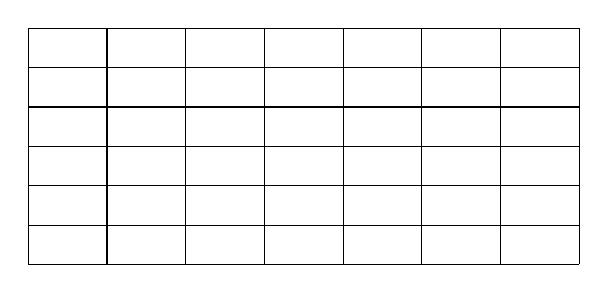
\begin{tikzpicture}[scale=0.5] 
            \draw (0,0) -- (0,6); 
            \draw (0,6) -- (14,6); 
            \foreach \i in {2,4,6,8,10,12,14} {
                \draw (\i ,6) -- (\i , 0); 
            } 
            \foreach \i in {1,2,3,4,5} {
                \draw (0, \i) -- (14, \i); 
            }
            \draw (0,0) -- (14,0);
        \end{tikzpicture}
    \end{center}
    \begin{solution} 
        We can count systematically by separating the problem into cases depending on the lengths of the rectangles, then breaking those cases into further cases depending on their heights.\footnote{Come to the Heights Folio Launch this Friday!} You could also 
        do it the other way around, but for this solution, let's consider doing it in this order.\begin{itemize} 
            \item Case 1: For rectangles with length 1, we can count 7 columns. Then, per column, we have 6 rectangles with height 1, 5 rectangles with height 2, and so on until we get 1 rectangle with height 6. Thus, we have $7\cdot(6+5+4+3+2+1) = 147$ rectangles. 
            \item Case 2: For rectangles with length 2, we can count 6 `columns'. Then, like the rectangles with length 7, there are 6 with height 1, and so on. Thus we have $6 \cdot (6+5+4+3+2+1) = 126$ rectangles. 
        \end{itemize} \begin{center} \vspace{-\parskip} $\vdots$ \end{center} \begin{itemize} 
            \item Case 7: For rectangles with length 7, there is only 1 `column'. Then, we have $6+5+4+3+2+1$ for all the differing heights. That gives us 21 rectangles. 
        \end{itemize} In summation notation, this is\[
            \sum_{i=1}^7 i (6+5+4+3+2+1) = \sum_{i=1}^7 21i.     
        \] Adding all the cases together gives us 588 rectangles in total. This problem is one that's a lot easier to explain with illustrations, and while I would normally 
        try to make TikZ pictures for it, I'm pressed for time. If you want a more visual explanation, just ask. 
    \end{solution} 
\end{enumerate} 

\end{document} 